\section{Data Processing Package - Structure}

Each data processing package has four folders (\texttt{Input\_files, Output\_files, \texttt{Log\_files,}} and \texttt{ Functions\_scripts}) and one file (\texttt{run.sh}). We can change the whole package name and transfer it to another location in the memory, or other computers. Once we choose a name to the internal folders, we can't change the name of the folders. This is because of using these folder names for handling the path. Each file and folder has a specific functionality.

\begin{figure} [ht]
\centering
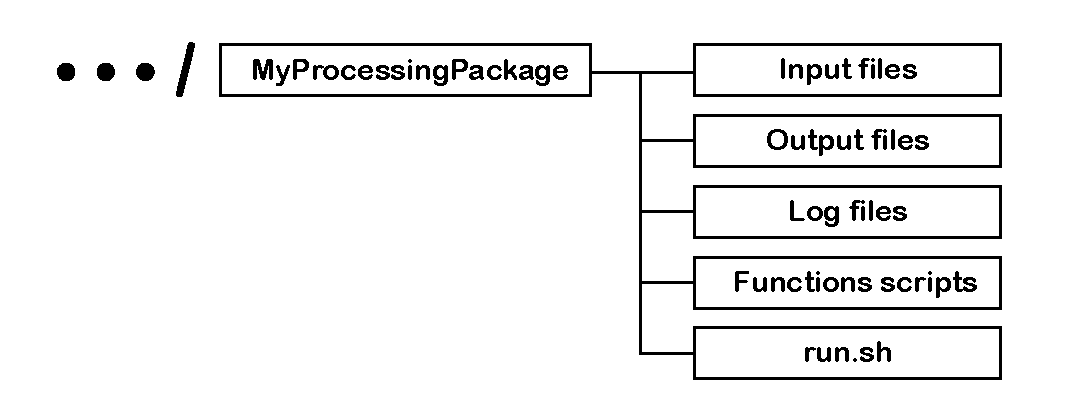
\includegraphics[scale=0.8]{figures/pdf/Figure02.pdf} 
\caption{File and folders of the data processing package.}
\label{fig:structure}
\end{figure}

\noindent
\texttt{Input\_files} folder includes all files (or folders) that we want to process. These files can be raw data, list of filenames, or results from other projects. \texttt{Output\_files} folder contains all files that we produce, it could be text files, figures, pdf files, and temporary files. \texttt{Log\_files} folder keeps files that help us to track the program's operation. It could be the history of runs (like, login info and time of running), report the success and failure for each set of data, and summary of the processing.  \texttt{Functions\_scripts} has all functions and scripts of Matlab and Shell (or any other programing languages).  \texttt{run.sh} is a shell script file that basically calls the other scripts and perform the whole processing sequence. This file is the right place to define necessary parameters to expand the functionality of the processing package. For example we can ask the program to keep data of all steps, report only a final pdf file, or ignore some steps.  \texttt{Log\_files} and  \texttt{Output\_files} are the only folders in which we can add, remove, or modify data. Even the core programs read data from  \texttt{Output\_files} folder. We will discuss more about this in the following sections.

